\chapter{Supervised Learning Method}
\label{ch:machine}

This chapter introduces the learning method used in this dissertation, includes random forest, linear regression, artificial neural network (ANN), supported vector machine (SVM) and logistic regression. Except ANN, other learning method are the native library of Spark MLlib.\\


An agent is learning if it can improve its performance on future tasks through current experience\cite{russell2003artificial}. In this study, the system can learn a model through previous stock price, and used to predict future changes.\\


Machine Learning algorithms can be classified into three groups\cite{russell2003artificial}, 
\begin{enumerate}
	\item \textit{Reinforcement learning}: the agent learns from a series of reinforcements-rewards or punishments. For example, an student learns to be punctual to school after get punished of late.
	\item \textit{Unsupervised learning}: Given a lot of data, let the agent itself to infer a function to description hidden information from those.
	\item \textit{Supervised learning}: This is the main algorithm using in this study. Every training data contains input variables (also called features), and its outcome (also called label). supervised learning learns from a set of such type data, to a function h (also called hypothesis).
\end{enumerate}


In this study, the label of every sample is tomorrow's stock price, changing direction or differential amount, the features are those parameters mentioned in Chapter~\ref{ch:market}.\\


When the target variable that we're trying to predict is continuous, e.g. predicting tomorrow's stock price, we call this type of problem as \textbf{regression} problem. On the other hand, if the target variable only have a small number of discrete values (such as stock price changing direction, up or down), we call it a \textbf{classification} problem.


\section{Linear Model}
Regression method are mainly used to predict stock price or its changing amount in combined system.

\subsection{Linear Regression}
Linear regression can be defined using the following equation,
\begin{equation}
	y=w^Tx + \varepsilon
\end{equation}
$ w $ is called \emph{weights}, and $ x $ is features vector, y is target variable, and $ \varepsilon $ is called error term. One example of linear regression can be found in figure~\ref{fg:linear_regression}. This algorithm assumes that the relationship between features and label follows a linear model.
\begin{figure}[h]
	\centering
	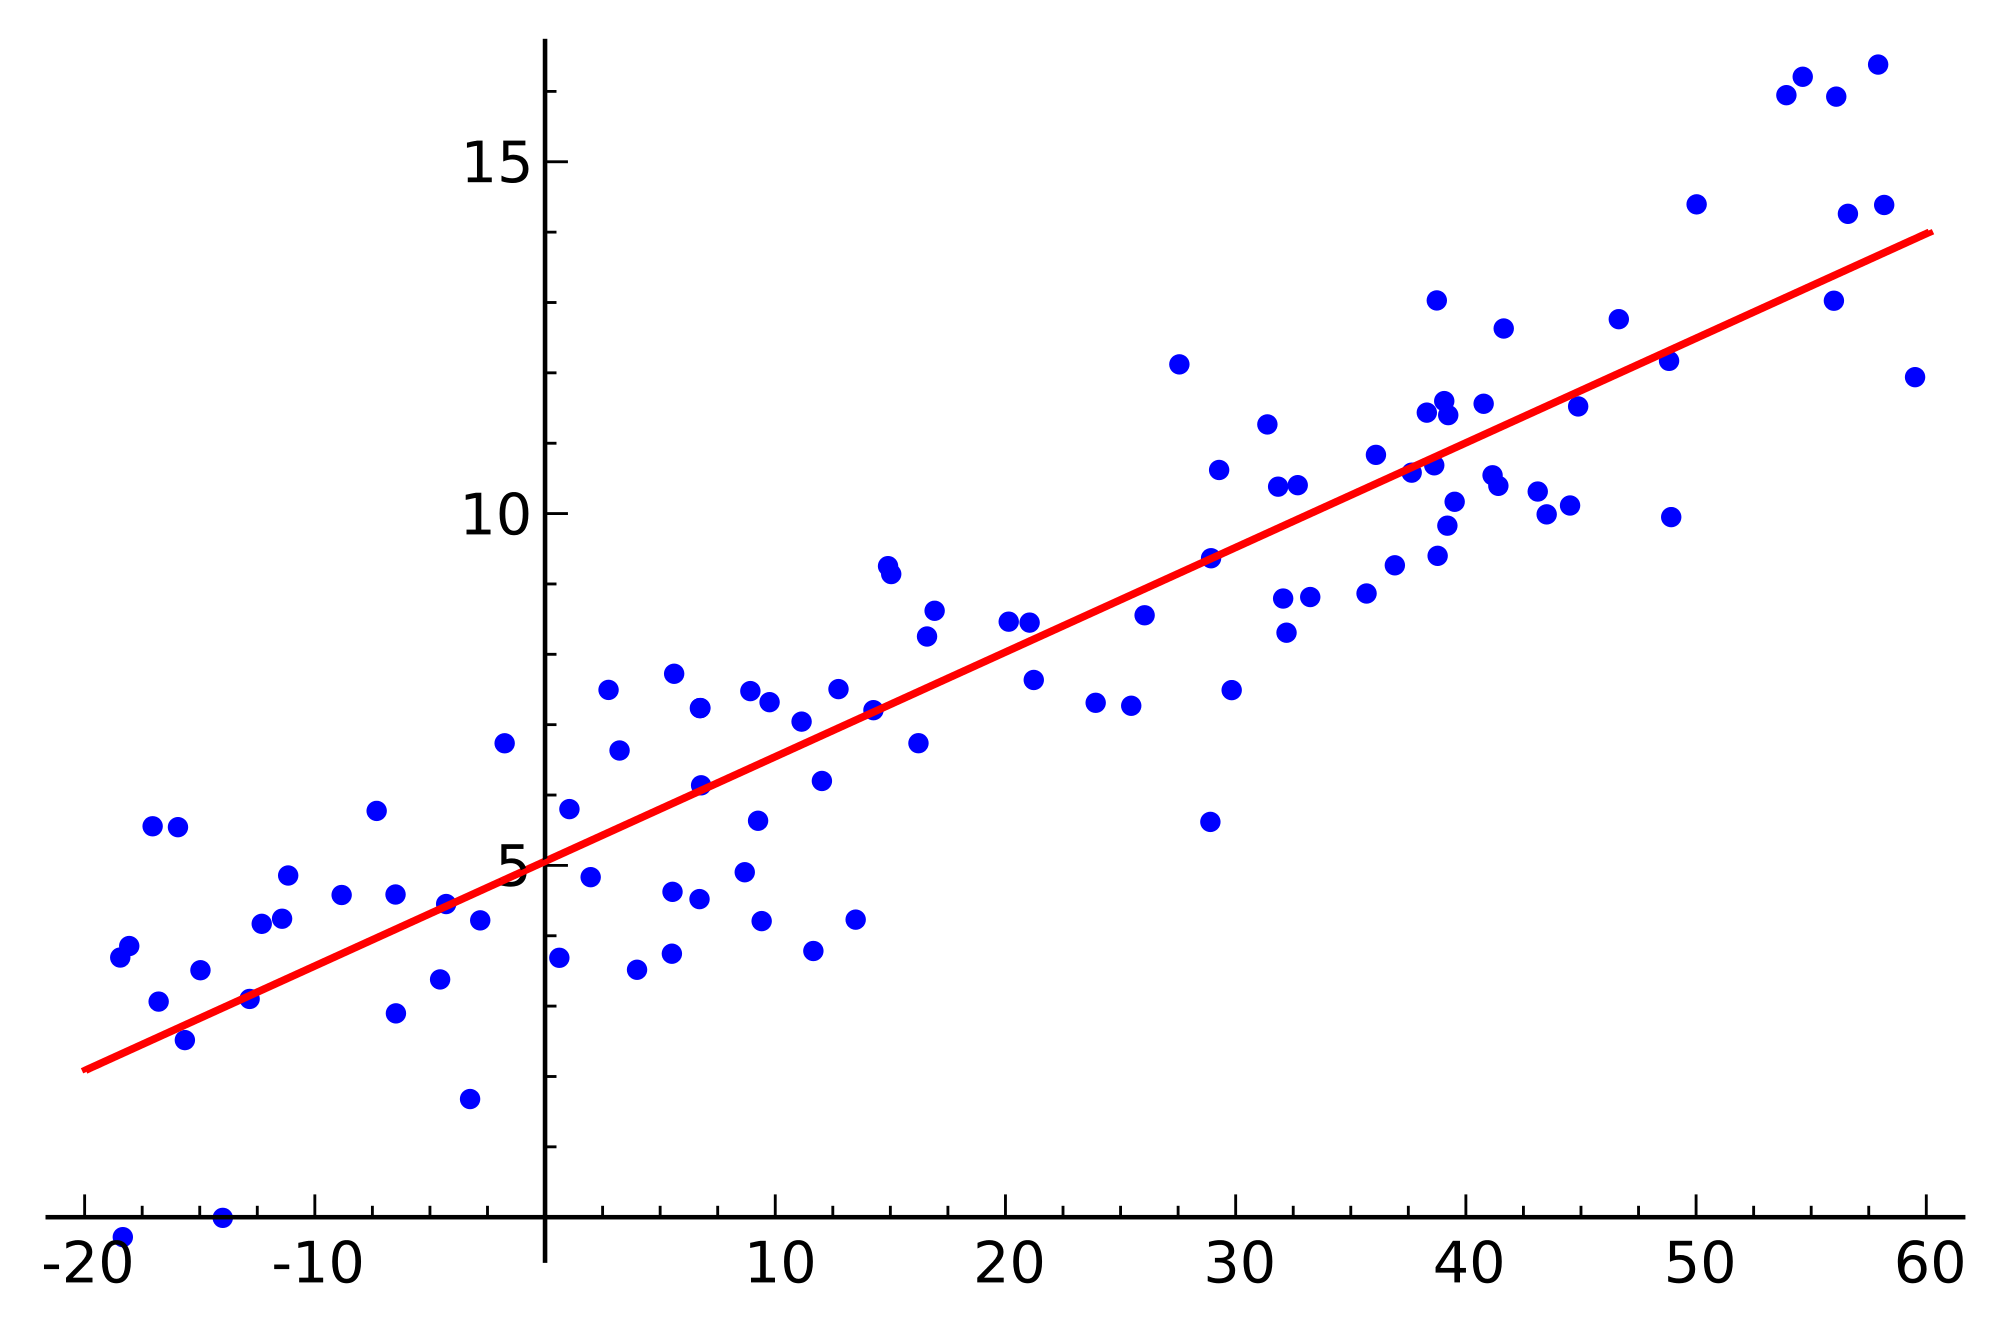
\includegraphics[width=0.6\textwidth]{Linear-regression}
	\caption{Example of simple linear regression with one variable}
	\label{fg:linear_regression}
\end{figure}


There are a large number of procedures which have been developed for parameters estimation and inference in linear regression. Spark MLlib uses least-square estimation\cite{7_mllib_linear_methods}.\\


Given a training set $ (x, y) $ (set number is $ n $), and initial weights $ w $, the error is computed as
\begin{equation}
error := \frac{1}{2} (w^T x - y)^2.
\label{eq:error_equation}
\end{equation}
This type of error is known as mean squared error (MSE).\\


After known the error, next step is using \emph{gradient descent} algorithm to update weight. Update equation is,
\begin{equation}
w_i=w_i-\alpha \frac{\partial}{\partial w_i} error
\label{eq:update_equation}
\end{equation}
Here $ \alpha $ is called learning rate. 


From above equation we can get that,
\begin{equation}
\begin{split}
\frac{\partial }{\partial w_i} error & = \frac{\partial }{\partial w_i} \frac{1}{2}(w^Tx-y)^2\\
& = 2 \cdot \frac{1}{2} (w^Tx-y) \cdot \frac{\partial }{\partial w_i} (w^Tx-y)\\
& = (w^Tx-y) * \frac{\partial }{\partial w_i} (\sum_{j=0}^{n}w_j x_j - y)\\
& = (w^Tx-y)x_i
\end{split}
\label{eq:partil_error}
\end{equation}


Then the updating rule becomes
\begin{equation}
w_i = w_i + \alpha (w^Tx-y)x_i
\end{equation}

This is gradient descent, also called batch gradient descent, the illustration is as figure~\ref{fg:gradient_descent}
\begin{figure}[h]
	\centering
	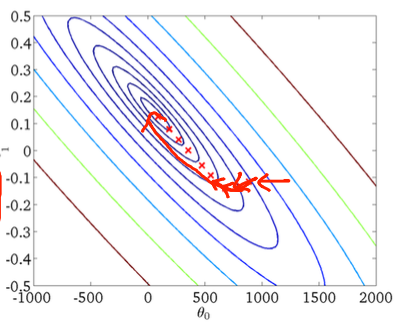
\includegraphics[width=0.6\textwidth]{steepest-descent}
	\caption{Illustration of gradient descent}
	\label{fg:gradient_descent}
\end{figure}

\clearpage
This algorithm runs very slow for a large data set input, as in every iteration, the errors of every data pair should be calculated.\\


Spark MLlib use \emph{stochastic gradient descent (SGD)} to speed up the training process\cite{7_mllib_linear_methods}.\\


The core idea of SGD is that updating parameters according to the gradient of the error with respect to that a small sample of training example (even one). The illustration of SGD can be found in figure~\ref{fg:SGD}
\begin{figure}[h]
	\centering
	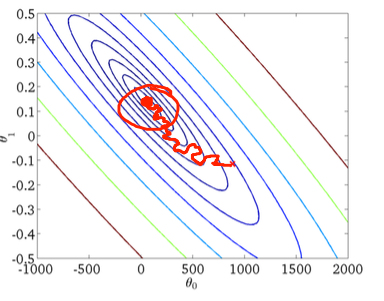
\includegraphics[width=0.6\textwidth]{sgd}
	\caption{Illustration of stochastic gradient descent (SGD)}
	\label{fg:SGD}
\end{figure}
Usually, SGD gets $ w $ "close" to the optimal solution more faster than batch gradient descent\cite{bottou2010large}, (but may never reach that solution), this makes SGD more suitable to large scale data regression.\\


In this study, the training iterations of our linear regression model are set to 100000, while the learning rate is 0.001.

\subsection{Linear Support Vector Machines (SVMs)}
SVMs was developed by Vladimir Vapnik\cite{cortes1995support} and is one of the most popular supervised learning methods. This study uses SVM to solve the classification of stock change direction, a typical 2-class classification problem.\\


Without loss of generality, let's using a simple 2-D example to illustrate this problem. Assume we have a set of data, and we want to classify them into two categorical classes. As figure~\ref{fg:SVM} shows, there exits two possible parting lines with different boundary sizes. Are these decision boundaries equally good?
\begin{figure}[h]
	\centering
	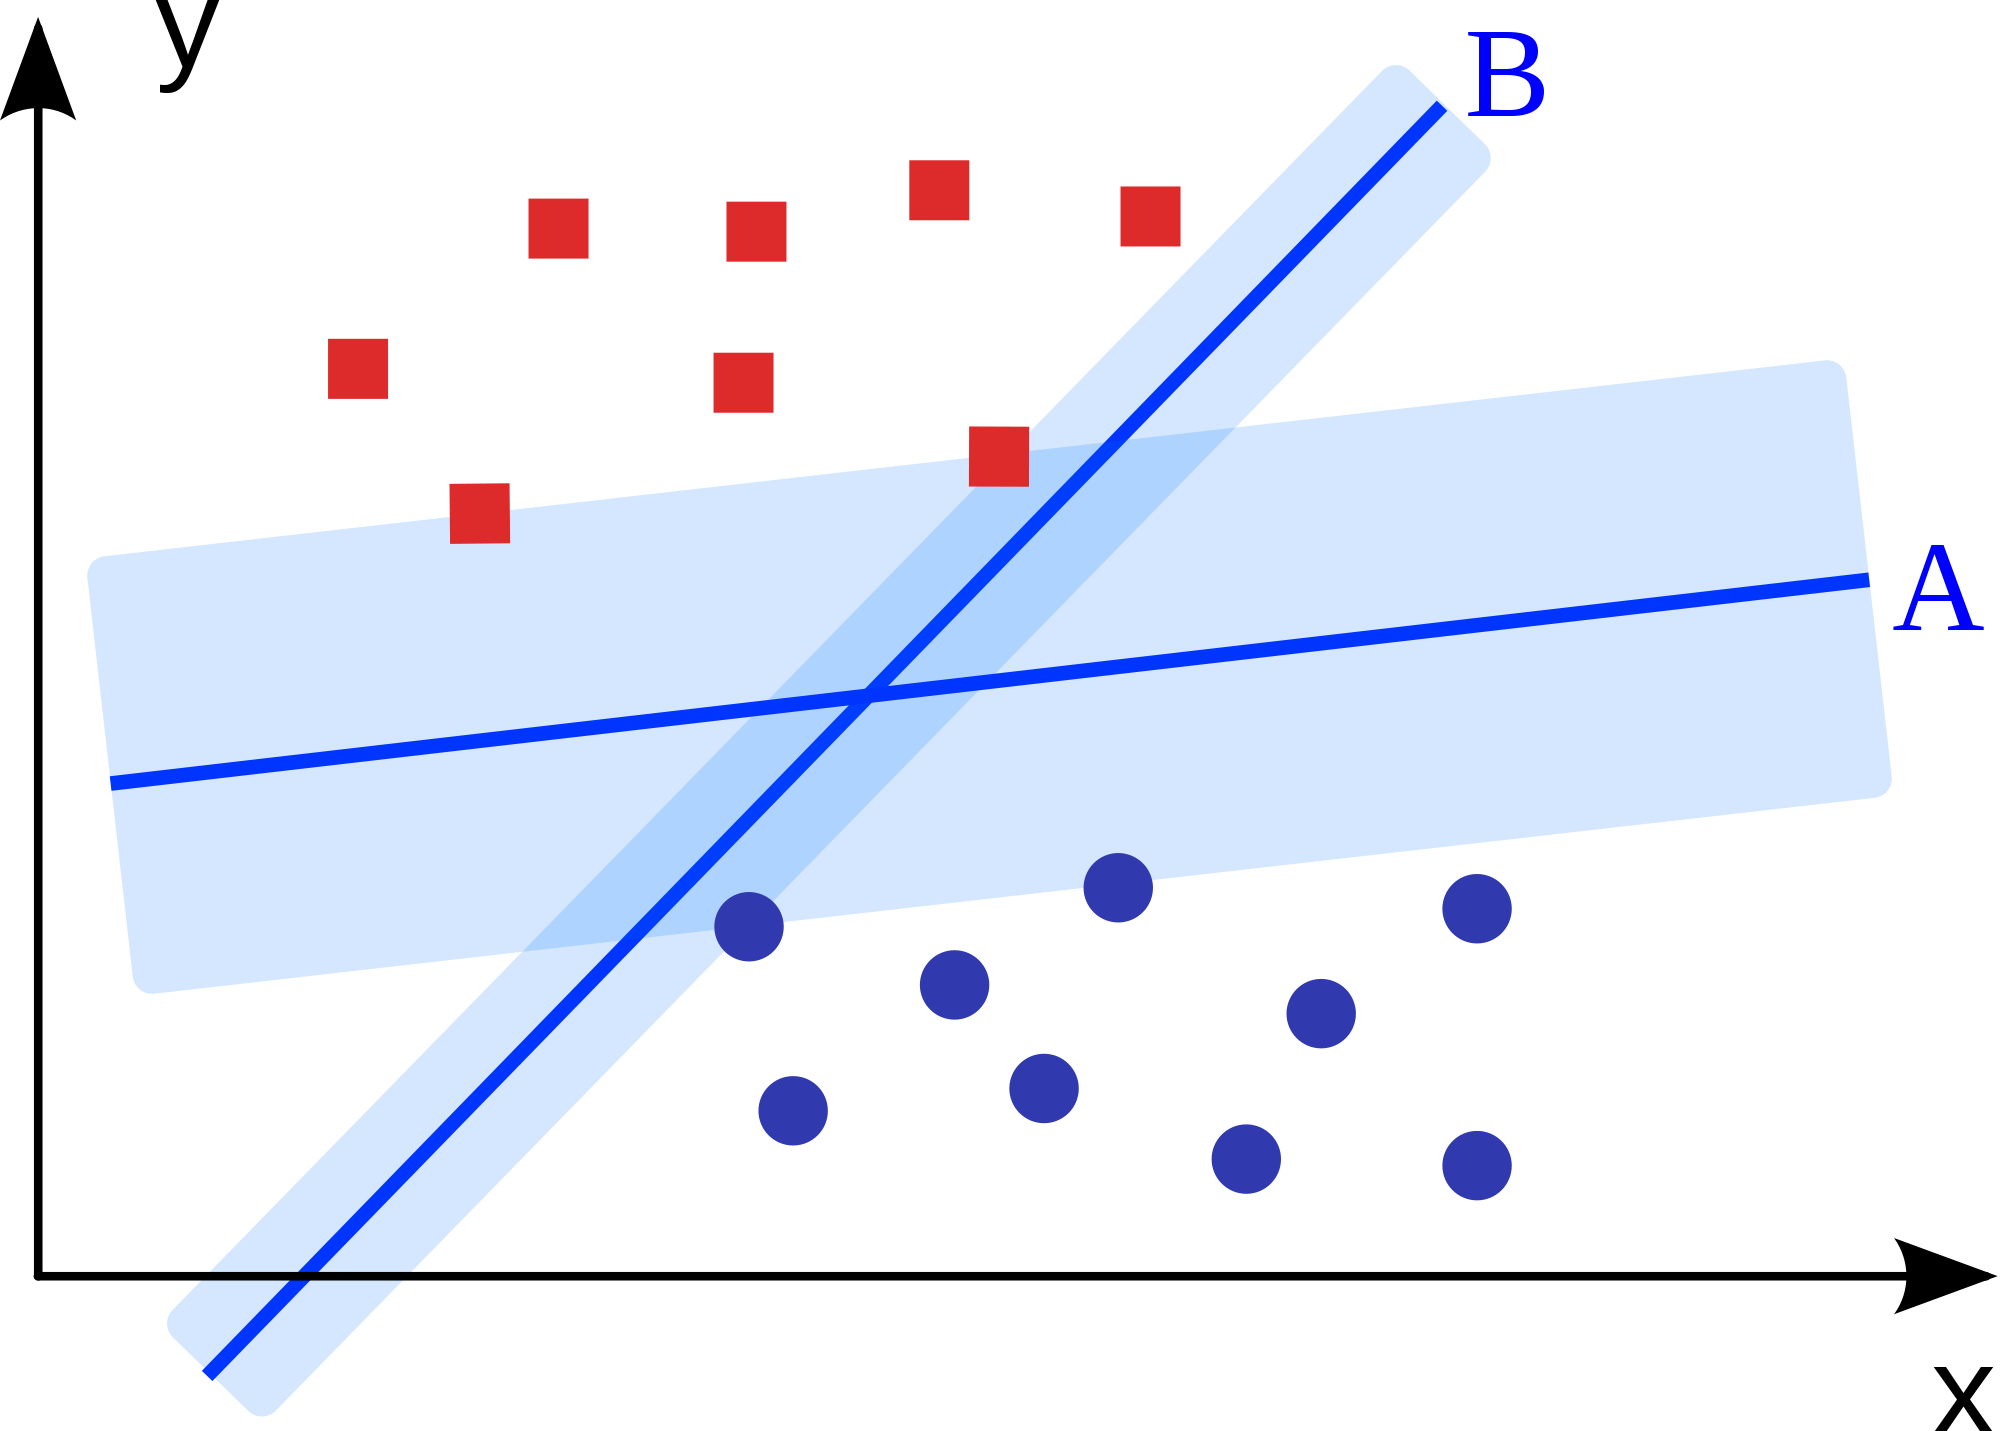
\includegraphics[width=0.8\textwidth]{svms}
	\caption{Illustration of service vector machines\cite{8_svm_2016}}
	\label{fg:SVM}
\end{figure}
\clearpage
The main idea of SVM is: "The decision boundary should be as far away as possible from the data points of both class"\cite{4_kantardzic}. Based one the above idea, A is a better parting line than B (in figure~\ref{fg:SVM}).\\


Mathematica description is as follows. Given a classification problem with a training set $ D $, belongs to two classes (using binary with -1 and 1)
\begin{equation}
D={(x_1,y_1),(x_2,y_2),\dots,(x_n,y_n)},x\in R^n, y\in{-1, 1},
\end{equation}
The hyperplane can be represented as
\begin{equation}
w^T \cdot x+b=0
\end{equation}
This means that
\begin{align*}
w^T\cdot x_i+b>0,& \text{if $y_i = 1$}\\
w^T\cdot x_i+b<0,& \text{if $y_i = -1$}
\end{align*}
Then margin can be mathematically expressed as the following equation\cite{6_tan_steinbach_kumar_2005}
\begin{equation}
margin=\min_{i=1,\dots,n}y_i\cdot(\frac{w^T\cdot x_i}{\lVert w\rVert} +\frac{b}{\lVert w\rVert})
\end{equation}
Then next step is to find the maximum margin.\\


However, in real-world applications, there are the cases where subsets cannot be completely separated (like figure~\ref{fg:SVM_soft})\cite{4_kantardzic}. In other words, the algorithm would find a balance between maximizing the margin and minimizing the classifications error during optimization process.
\begin{figure}[h]
	\centering
	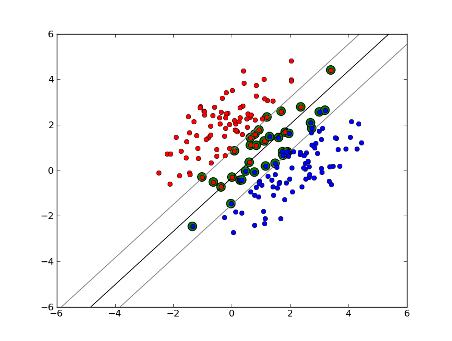
\includegraphics[width=0.8\textwidth]{svm_soft}
	\caption{Soft margin of SVMs}
	\label{fg:SVM_soft}
\end{figure}

\subsection{Logistic Regression}
Logistic is also a widely used method to predict binary responses. Rather than predicting the value of the dependent variable in linear regression, logistic regression method estimates the probability that the dependent variable will choose from a given range\cite{4_kantardzic}.

 
Logistic regression takes probabilities of every label into consideration. Suppose that output Y has two possible values, 0 and 1. In training set, the possibilities can be expressed as: $ P(y_i=0)=1-p_i $ and $ P(y_i=1)=p_i $, then the \textit{linear logistic model} can be represented by~\cite{4_kantardzic},
\begin{equation}
	\log (\frac{p_i}{1-p_i}) = b + w^T \cdot x_i
\end{equation}
The reason for using the logit form of output is to prevent the model from generating a result out-range of $ [0, 1] $\\


In this system, logistic regression algorithm are mainly used to predict the changing direction of stock price.

\section{Random Forest}
Random forest algorithm was first created by Tin Kam Ho\cite{ho1995random} and is based on decision trees. To reduce the risk of overfitting, random forests composes of a number of individual decision trees, and this is also where this method get its name from (as figure~\ref{fg:decision-tree} shows).
\begin{figure}[h]
	\centering
	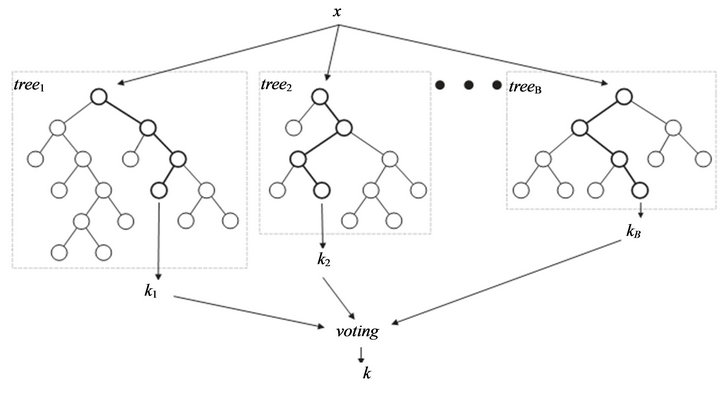
\includegraphics[width=0.9\textwidth]{random-forest}
	\caption{Illustration of random forest}
	\label{fg:decision-tree}
\end{figure}

\clearpage
Random Forest can solve both classification and regression problems. For the former problem, every decision tree's prediction is counted as a vote for one class, and the final result is the class that received most votes (like figure~\ref{fg:decision-tree}). For the later question, final result this the average of all decision trees' prediction value.\\


As every decision tree are trained and predicted separately, they can work in parallel, which makes random forest a very suitable algorithm for distributed computing.


\section{Artificial Neural Network}
Neural networks was first inspired by human nervous system which is made up of neurons, a information processing unit (figure~\ref{fg:neural-nework}). Every neuron receive signals from input or former neurons, then compute them with the activation function and send its result to output or latter neurons\cite{russell2003artificial}.
\begin{figure}[h]
	\centering
	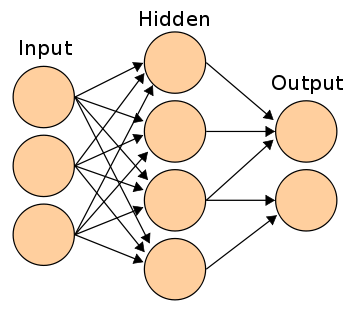
\includegraphics[width=0.6\textwidth]{neural_network}
	\caption{Illustration of Artificial Neural Network with one hidden layer}
	\label{fg:neural-nework}
\end{figure}

This study focus on back propagation MLP. The steps of algorithm can be described as follow\cite{russell2003artificial}:
\begin{enumerate}
	\item \textit{Initialize weights $ w $ with a small random value}. Suppose layer $ j $ has $ m $ nodes, layer $j + 1$ has $ n $ nodes, then the weight matrix between these two layer $ w_{jj+1} $ should have $ m \times n $.
	\item \textit{Forward Propagation}. The values of every layer $ i $ remark as $ l_i $ (Input as $ l_i =l_1 $, output as $l_o=l_n$, suppose there are n layers in total), the node $ k $ in $ l_j $ remark as $ l_jk $. Given the activation function
	\begin{equation}
	f(l) = \frac{1}{1+e^{-l}}
	\end{equation}
	the value of layer $ i + 1 $ is calculated by,
	\begin{equation}
	l_{i+1}=f(w_{ii+1}^T\cdot l_i)
	\end{equation}
	From the input layer, do this calculation. Record those values as $ l = [l_i, l_2, \ldots, l_o] $.
	\item \textit{Back Propagation and weights update} 
	\begin{enumerate}
		\item Get the error value using
		\begin{equation}
		\delta_n = y - l_n
		\end{equation}
		
		\item For the following layers, using formula,
		\begin{equation}
		\delta_j = w_{jj+1}^T\delta_{j+1}\cdot f'(l_i)
		\end{equation}
		where $ f'(l) = f(l)(1-f(l)) $
		
		\item Update weights.
		\begin{equation}
		w_{ii+1} = w_{ii+1} + \alpha \delta_i 
		\end{equation}
	\end{enumerate}
\end{enumerate}

The above algorithm is a typical batch gradient descent process. As data amount is relatively small (e.g. 1 year only have around 250 transaction days), using this method is much faster to reach the optimal solution.

\section{Summary}
This chapter introduces the learning algorithms used in this study. The regression method (Random Forest, ANN, Linear Regression) are used to predict the stock price directly or the changing amount, while the classification method (Logistic Regression, SVM, Random Forest) are used to predict the change direction.